\fbox{
\algoblock{0.55}{\scriptsize Merge Sort}{
    \scriptsize
    \begin{minipage}[t]{0.6\textwidth}
    \begin{enumerate}[noitemsep]
        \item \textbf{Divide}: Split the array evenly into two smaller subarrays, and continue dividing recursively.
        \item \textbf{Sort (Recursively)}: Apply merge sort recursively on each subarray until each has only one element (base case).
        \item[] 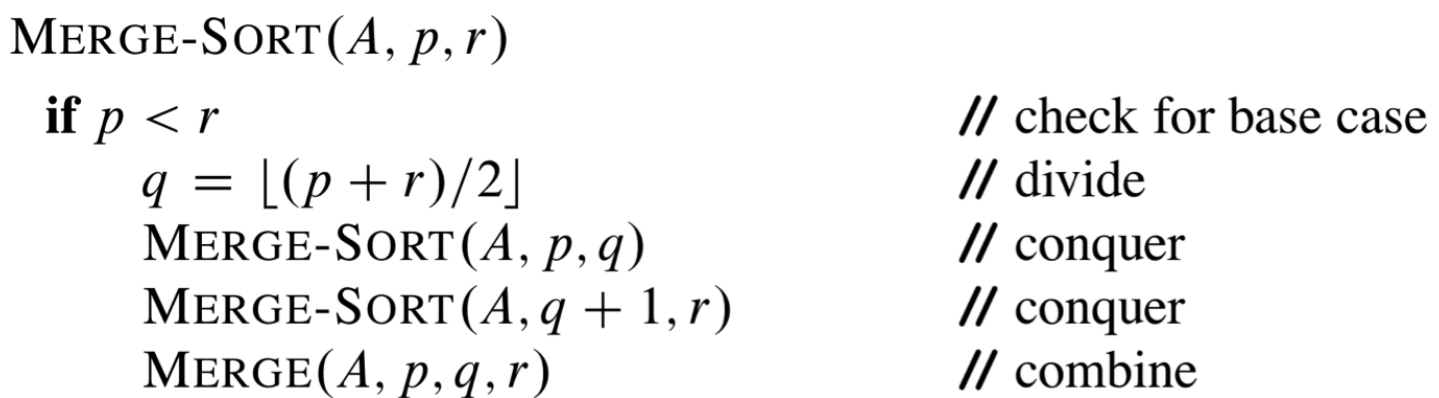
\includegraphics[width=0.75\linewidth]{images/merge-sort.png}

        \item \textbf{Merge}: Combine the two sorted subarrays into a single sorted array:
        \begin{enumerate}[noitemsep]
            \item Initializing pointers at the start of each subarray.
            \item Comparing the elements pointed to, and appending the smaller one into a new array.
            \item Advancing the pointer in the subarray from which the element was chosen.
            \item Repeating this process until all elements in both subarrays are merged into the sorted array.
        \end{enumerate}
    \end{enumerate}
    \justifying
    \textit{Merge Cost Complexity:} \(O(n)\) per merge operation.\\
    \textit{Time Complexity:} \(O(n \log n)\) \quad \textit{Space Complexity:} \(O(n)\)
    \end{minipage}
    \hfill
    \begin{minipage}[t]{0.35\textwidth}
        \vspace{0pt}
        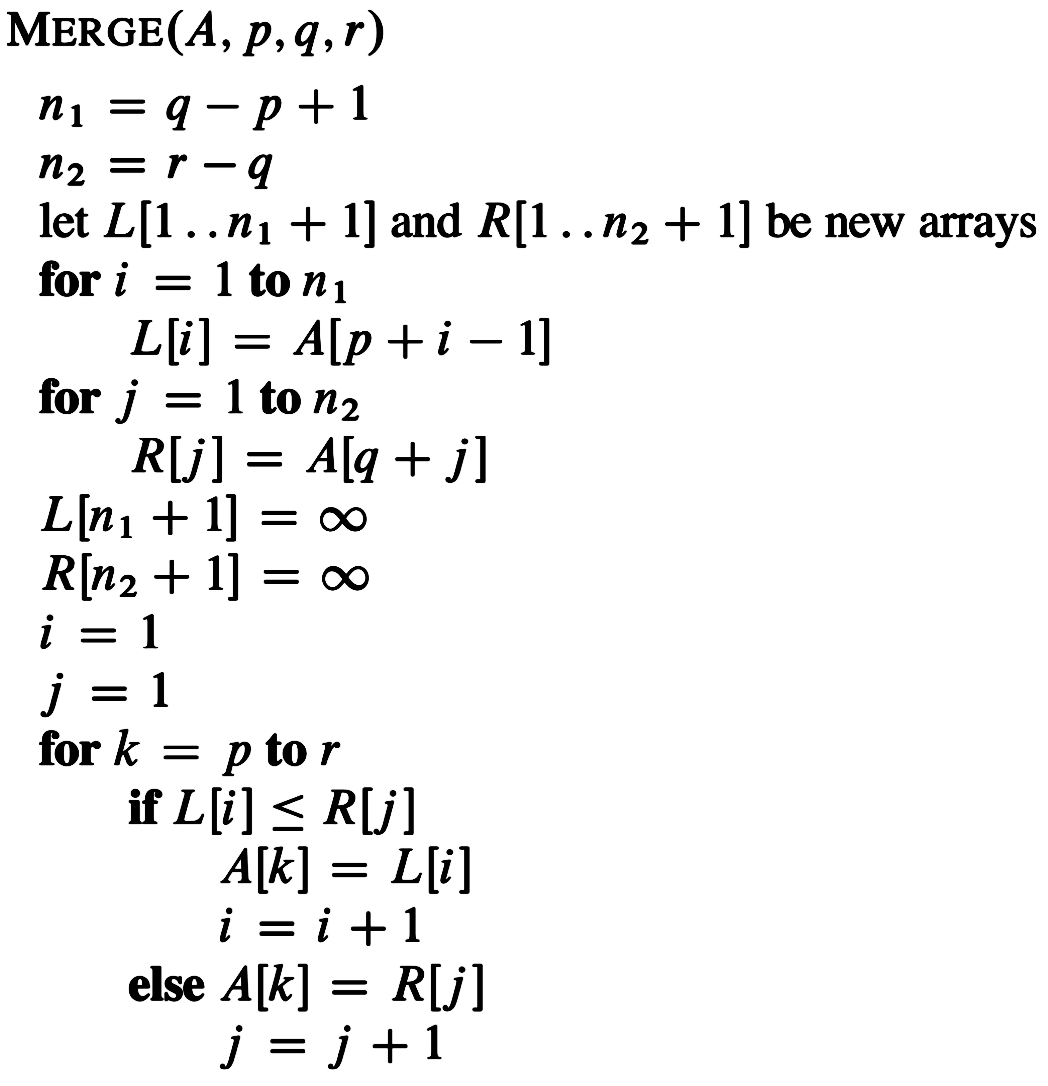
\includegraphics[width=1\linewidth]{images/merge.png}
    \end{minipage}
}
} 